\begin{enumerate}
\item 
\[ \sum_{\substack{p\leq x\\p=k \bmod l}}\frac{\log p}{p} = \frac{1}{\phi(l)}\log x + \frac{1}{\phi(l)}\sum_{\chi\neq\1}\overline{\chi(k)}\underbrace{\sum_{p\leq x}\frac{\chi(p)\log p}{p}} + O(1) \]
\item
\[ \sum_{p\leq x}\frac{\chi(p)\log p}{p} = \sum_{n\leq x}\frac{\chi(n)\Lambda(n)}{n} + O(1) \]
\item
\[ \sum_{n\leq x}\frac{\chi(n)\Lambda(n)}{n} = k\sum\frac{\chi(n)\mu(n)}{n} + O(1)\co\quad k=k_x=\sum_{n=1}^\infty\frac{\chi(n)\log n}{n} \]
\end{enumerate}
\textbf{Step 4.}
\begin{align*}
\sum_{\substack{c,d\\cd\leq x}}\frac{\chi(c)\mu(c)}{c}\frac{\chi(d)}{d}
&= \sum_{n\leq x}\sum_{c\div n}\frac{\chi(n)}{n} \mu(k) \\
&= \sum_{n\leq x}\frac{\chi(n)}{n}\underbrace{\sum_{c\div n}\mu(c)}_{\text{$=1$ only when $n=1$}} \\
&= \frac{\chi(1)}{1} = 1
\end{align*}
\begin{align*}
1 &= \sum_{c\leq x}\sum_{d\leq x/c}\frac{\chi(c)\mu(c)}{c}\frac{\chi(d)}{d} \\
&= \sum_{c\leq x}\frac{\chi(c)\mu(c)}{c}\sum_{d\leq x/c}\frac{\chi(d)}{d} \\
&= \sum_{c\leq x}\frac{\chi(c)\mu(c)}{c}(L+g(x)) \\ \intertext{where $L=\sum_{n=1}^\infty\frac{\chi(n)}{n}$, $\abs{g(x)}\leq\phi(l)\frac cx$}
&= L\sum_{c\leq x}\frac{\chi(c)\mu(c)}{c} + \sum_{c\leq x}\frac{\chi(c)\mu(c)g(x)}{c}
\end{align*}
We have
\begin{align*}
\abs[\Big]{\sum_{c\leq x}\frac{\chi(c)\mu(c)g(x)}{c}} &\leq \sum_{c\leq x}\frac{\phi(l)\frac cx}{c} \\
&= \frac{\phi(l)}{x} \sum_{c\leq x} 1 = \frac{\phi(l)}{x} (x+O(1)) = O(1) \\
\therefore L\cdot\sum\frac{\chi(n)\mu(n)}{n} &= O(1),
\end{align*}
where $L=L_x=\sum_{n=1}^\infty\frac{\chi(n)}{n}$.  It suffices to show that $L=L_x\neq0$, for all $\1\neq\chi\in\hat U_l$. (4)

\remark Dirichlet used the holomorphic function $L_x(z)$ defined for $\Re(z)>1$ by
\[ L_x(z) = \sum_{n=1}^\infty \frac{\chi(n)}{n^z} . \]
If we differentiate term by term, we get
\[ L'_x(z) = - \sum_{n=1}^\infty \frac{\chi(n)\log n}{n^z} \footnote{Aside:
\begin{gather*}
\paren[\Big]{\frac{1}{n^z}}' = (e^{-z\log n})' = -\log n \, e^{-z\log n} = \frac{-\log n}{n^z} \\
\intertext{We have } L_x(1) = \sum_{n=1}^\infty \frac{\chi(n)}{n} = L_x \\
L'_x(1) = -\sum \frac{\chi(n)\log n}{n} = - K_x
\end{gather*}
}\]
\textbf{Step 5(a):} Consider a real-valued character $\chi$, $\1\neq\chi\in\hat U_l$
\[ \chi\colon \Z \to \brace{0,\pm1} . \]
Let $A(n)=\sum_{d\div n}\chi(d)$, $B(x)=\sum_{n\leq x}\frac{A(n)}{\sqrt n}$. \\
We show that $B(x)\to\infty$, and $B(x)=\sqrt xL+O(1)$, so that $L\neq0$.

Since $\chi$ is (completely) multiplicative, $A$ is multiplicative. \\
(proof: for $a$, $b$ with $\gcd(a,b)=1$, each $d\div ab$ can be expressed uniquely as $d=kl$ with $k\div a$, $k\div b$, so:
\[ A(ab) = \sum_{d\div ab}\chi(d) = \sum_{k\div a}\sum_{l\div b}\chi(kl) = \sum_{k\div a}\chi(k)\sum_{l\div b}\chi(l) = A(a)A(b) . \]
So we have $A(\prod p_i^{k_i})=\prod A(p_i^{k_i})$ \\
We have
\[ A(p^m) = \sum_{d\div p^m}\chi(d) = 1 + \chi(p) + \chi(p)^2 + \dotsb + \chi(p)^m \]
If $\chi(p)=0$, then $A(p^m)=1$ \\
If $\chi(p)=1$, then $A(p^m)=1+m$ \\
If $\chi(p)=-1$, then $A(p^m)=\begin{cases}
1 & \text{if $m$ is even} \\
0 & \text{if $m$ is odd}
\end{cases}$ \\
$\therefore A(p^m)\geq0$ for all $p$, $m$, and if $m$ is even, $A(p^m)\geq1$. \\
$\therefore A(n)\geq0$ for all $n\in\Z^+$, with $A(n)\geq1$ when $n$ is a square.
\begin{gather*}
\therefore B(x) = \sum_{n\leq x}\frac{A(n)}{\sqrt n} \geq \sum_{n=m^2\leq x}\frac{A(m^2)}{m} \geq \sum_{m\leq\sqrt x}\frac1m \to \infty\text{, as $x\to\infty$.} \\
\text{\emph{Also,}}\qquad B(x) = \sum_{n\leq x}\frac{A(n)}{\sqrt n} = \sum_{n\leq x}\sum_{d\div n}\frac{\chi(d)}{\sqrt n} = \sum_{\substack{c,d\\cd\leq x}}\frac{\chi(d)}{\sqrt{cd}} \\
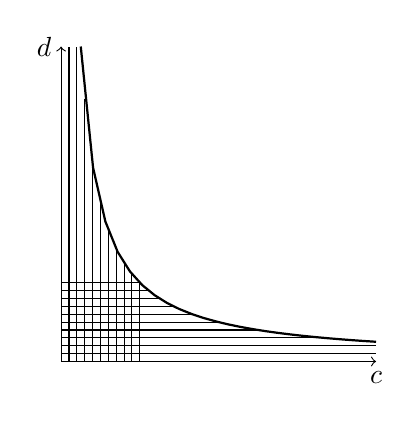
\begin{tikzpicture}
\draw[<->](0,4)--(0,0)--(4,0);
\node[left]at(0,4){$d$};
\node[below]at(4,0){$c$};
\draw[thick,domain=0.25:4] plot(\x,1/\x);
\foreach\x in{0.1,0.2,...,1}\draw(\x,0)--(\x,{min(4,1/\x)});
\foreach\x in{0.1,0.2,...,1}\draw(0,\x)--({min(4,1/\x)},\x);
\end{tikzpicture} \\
= \sum_{c\leq\sqrt x}\sum_{d\leq x/c}\frac{\chi(d)}{\sqrt{cd}} + \sum_{d\leq x}\sum_{c\leq x/d}\frac{\chi(d)}{\sqrt{cd}} - \sum_{c\leq\sqrt x}\sum_{d\leq\sqrt x}\frac{\chi(d)}{\sqrt{cd}} = \dotsb = \sqrt x L + O(1) %\\
\end{gather*}
\begin{align*}
\recall \qquad \sum_{n\leq x}\frac1{\sqrt n} &= f(1) + \int_1^x f(t)\d t + \int_1^x \chev{t} f'(t)\d t - \chev{x}f(x) , \\ \intertext{for $f(t)=t^{-1/2}$, $f'(t)=-\frac12t^{-3/2}$, $\int f=2t^{1/2}$.}
&= 1 + \int_1^x \frac1{\sqrt t}\d t - \int_1^x \frac{\chev{t}}{2^{3/2}} \d t - \frac{\chev{x}}{\sqrt x} \\
&= 1 + \brack[\Big]{2\sqrt t}_1^x - \int_1^\infty \frac{\chev{t}}{2t^{3/2}} \d t + \int_2^\infty \frac{\chev{t}}{2t^{3/2}} \d t - \underbrace{\frac{\chev{x}}{\sqrt x}}_{\mathclap{\in[0,1/\sqrt x)}} \\
&= 1 + 2\sqrt x - 2 - a + g(x) \\
&= 2\sqrt x + c + g(x),
\end{align*}
where $c=-1-\int_1^\infty\frac{\chev t}{2t^{3/2}}\d t$, and we have
\[ \abs[\Big]{\int_x^\infty\frac{\chev{t}}{2t^{3/2}}\d t} \leq \int_x^\infty \frac{1}{2t^{3/2}} \d t = \brack[\Big]{-\frac{1}{\sqrt t}}_x^\infty = \frac1{\sqrt x} , \]
so that $\abs{g(x)}\leq\frac{1}{\sqrt x}$
\begin{gather*}
(\therefore) \sum_{n\leq x}\frac1{\sqrt n} = 2\sqrt x + c + O\paren[\Big]{\frac1{\sqrt x}} . \\
\sum_{c\leq\sqrt x}\frac1{\sqrt c}\sum_{d\leq x/c}\frac{\chi(d)}{\sqrt d} = \sum_{c\leq x}\frac{1}{\sqrt c}\paren[\Big]{M+h\paren[\Big]{\frac xc}} , \\
\text{where}\qquad M = \sum_{n=1}^\infty \frac{\chi(n)}{\sqrt n},\qquad \text{and}\qquad \abs[\Big]{h\paren[\Big]{\frac xc}} \leq \phi(l) \sqrt{\frac{x}{c}} \\
= M \sum_{c\leq\sqrt x}\frac1{\sqrt c} + \sum_{c\leq\sqrt x}\frac{h(\frac xc)}{\sqrt c} = M(2x^{1/4}+O(1)) + O(1) , \\
\begin{aligned}
\text{since}\qquad \abs[\Big]{\sum_{c\leq\sqrt x}\frac{h(\frac xc)}{\sqrt c}} &\leq \sum_{c\leq\sqrt x}\frac{\phi(l)\sqrt{\frac cx}}{\sqrt c} \\
&= \frac{\phi(l)}{\sqrt x} \sum_{c\leq\sqrt x}1 = \frac{\phi(l)}{\sqrt x}(\sqrt x+O(1)) = O(1) \\
\therefore \sum_{c\leq\sqrt x}\sum_{d\leq x/c}\frac{\chi(d)}{\sqrt{cd}} &= 2Mx^{1/4} + O(1) .
\end{aligned}
\end{gather*}
\begin{align*}
\sum_{d\leq\sqrt x}\sum_{c\leq x/d}\frac{\chi(d)}{\sqrt{cd}} &= \sum_{d\leq\sqrt x}\frac{\chi(d)}{\sqrt d}\sum_{c\leq x/d}\frac{1}{\sqrt c} = \sum_{d\leq\sqrt x}\frac{\chi(d)}{\sqrt d}\paren[\Big]{2\sqrt{\frac xd}+O(1)} \\
&= 2\sqrt x\sum_{d\leq\sqrt x}\frac{\chi(d)}{d} + \sum_{d\leq x}\frac{\chi(d)}{\sqrt d}O(1) \\
&= 2\sqrt x(L+O(\tfrac1{\sqrt x})) + O(1)(M+O(\tfrac1{x^{1/4}})) \\
&= 2\sqrt xL+O(1) .
\end{align*}
\begin{align*}
\sum_{c\leq\sqrt x}\sum_{d\leq\sqrt x}\frac{\chi(d)}{\sqrt{cd}} &= \paren[\Big]{\sum_{c\leq\sqrt x}\frac1{\sqrt c}}\paren[\Big]{\sum_{d\leq\sqrt x}\frac{\chi(d)}{\sqrt d}} \\
&= (2x^{1/4}+O(1))(M+O(\tfrac1{\sqrt c})) = 2Mx^{1/4} + O(1) .
\end{align*}
\begin{align*}
\therefore B(x) &= \sum_{c\leq\sqrt x}\sum_{d\leq x/c}\frac{\chi(d)}{\sqrt{cd}} + \sum_{d\leq\sqrt x}\sum_{c\leq x/d}\frac{\chi(d)}{\sqrt{cd}} - \sum_{c\leq\sqrt x}\sum_{d\leq\sqrt x}\frac{\chi(d)}{cd} \\
&= (2Mx^{1/4}+O(1)) + (2\sqrt xL+O(1)) - (2Mx^{1/4}+O(1)) \\
&= 2\sqrt x L + O(1) .
\end{align*}
